\section{Implementación}

{
\setbeamercolor{background canvas}{bg=beamer@blendedblue!30}
\begin{frame}
  % frame contents here
    \centering
  \Huge
  Implementación
\end{frame}
}

\begin{frame}
    \frametitle{Arquitectura}
    \begin{columns}[T] % Align columns at the top
        \begin{column}{0.6\textwidth}
          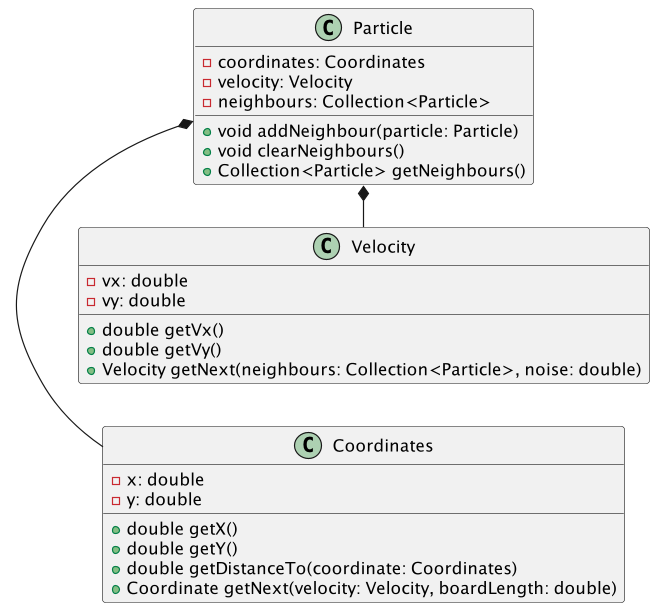
\includegraphics[width=\textwidth]{images/particle-diagram.png} 
        \end{column}
        \begin{column}{0.4\textwidth}
            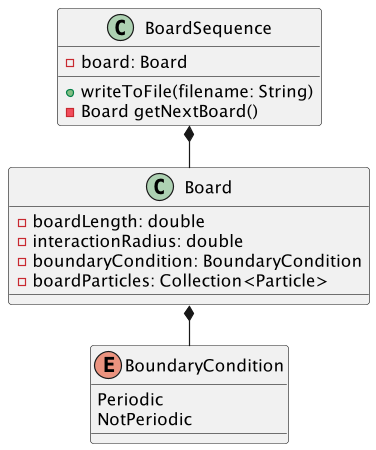
\includegraphics[width=\textwidth]{images/board-diagram.png} 
        \end{column}
    \end{columns}
\end{frame}

\begin{frame}
    \frametitle{Motor de simulación}
    \begin{block}{}
        Utiliza el método getNextBoard de la clase BoardSequence para avanzar en el tiempo y obtener el próximo Board.
    \end{block}

    \large Resumen de las operaciones realizadas:
    \begin{itemize}
            \item Cálculo de la nueva velocidad y posición 
            \item Se actualiza la velocidad y posición de la partícula
            \item Se recalcula las celdas en las que se encuentran las partículas
            \item Se obtienen los vecinos utilizando Cell Index Method
    \end{itemize}
    
\end{frame}

% \begin{frame}
%     \frametitle{Actualización de posición}
% \begin{lstlisting}[style=pseudocode, caption={Pseudocódigo para función getNext de clase Coordinates}]
% Function getNext(v: Velocity, boardLength: Real) -> Coordinates:

%     nextX = this.x + v.x
%     nextY = this.y + v.y
    
%     // wrapAxis es una funcion auxiliar que considera la condicion periodica de borde
%     nextX = wrapAxis(nextX, boardLength)
%     nextY = wrapAxis(nextY, boardLength)

%     return Coordinates(nextX, nextY)
% \end{lstlisting}

% \end{frame}

\begin{frame}[fragile]{Actualización de la posición}
  \begin{lstlisting}
Function getNext(v: Velocity, boardLength: Real) -> Coordinates:

    nextX = this.x + v.x
    nextY = this.y + v.y
    
    // se considera la condicion periodica de borde
    nextX = wrapAxis(nextX, boardLength)
    nextY = wrapAxis(nextY, boardLength)

    return Coordinates(nextX, nextY)
  \end{lstlisting}
\end{frame}

\begin{frame}[fragile]{Actualización de la velocidad}
  \begin{lstlisting}
getNext(neighbours: list<particle>, noise: double) -> Velocity:
    noiseValue = RandomBetween(-noise/2, noise/2)
    
    angles = new list
    for each particle IN neighbours:
        angle = arctan(particle.vy / particle.vx)
        angles.add(angle)

    selfAngle = arctan(this.velocity.y / this.velocity.x)
    angles.add(selfAngle)

    sinAvg = promedio de los senos en 'angles'
    cosAvg = promedio de los cosenos en 'angles'

    nextAngle = arctan(sinAvg / cosAvg) + noiseValue
    nextVx = cos(nextAngle) * modulo de v
    nextVy = sin(nextAngle) * modulo de v

    return Velocity(nextVx, nextVy)
  \end{lstlisting}
\end{frame}